% Chapter 1
%\chapter{The Standard Model of Particle Physics}\label{Chapter1} % Main chapter title
\chapter{Theoretical Background}\label{Chapter1} % Main chapter title
\section{The Standard Model}\label{chapter1_sec1_SM}
The main goal of particle physics is to fully understand the nature of the constituents of the matter and the fundamental 
forces through which they interact. There are many theories purposed to understand the physics laws at particle level but the Standard 
Model(SM) is the one which stood firm against high precision tests~\cite{Reference1}. It is a collaborative theory of
fundamental world, developed in 20th century which can express the fundamental particles (bosons and fermions) and the underlying
interactions with the concept of mediating gauge bosons. The last unverified part of the SM, the Higgs boson, was discovered in 2012 at LHC of European Organization for Nuclear Research(CERN)~\cite{Reference20,Reference21}.  Despite of incredibly successful theory of particle world, the SM does fail to fully describe the known universe.
%\par This chapter is structured as follows. Details of the fundamental particles and the interactions would be described
%in Section~\ref{chapter1_sec1}. The Higgs mechanism, Higgs boson production 
%and decays at LHC would be described in Sections~\ref{chapter1_sec2}~and~\ref{chapter1_sec3}. Experimental Observations
%of the Standard Model would be described in 
%Section~\ref{chaper1_sec4}. Physics beyond the Standard Model will be described in Section~\ref{chapter1_sec5}.  
 % For referencing the chapter elsewhere, use \ref{Chapter1} 

%----------------------------------------------------------------------------------------
\section{Fundamental Particles and underlying Interactions}\label{chapter1_sec1}
\subsection{Fundamental Particles}
Particle with unknown structure is called fundamental particle. Fundamental particles can be categorized into fermions (characterized by Fermi-Dirac statistics) and bosons (Bose-Einstein statistics). 
%Particles which are characterized by Fermi-Dirac statistics and Bose-Einstein statistics are called fermions and bosons respectively. 
The spin-statistics theorem classifies the particles with integral spin as bosons, while particles with half-integral spin as fermions. Fermions includes all leptons, quarks and baryons (composite particles three  quarks). 
Ordinary matter is composed of leptons and quarks which are categorized in three ``generations'' as illustrated in Table \ref{table:quarks_leptons}. 
First generation includes an ``up'' type quark which carries electric charge $+\frac{2}{3}$ and a ``down'' type quark carrying electric charge
$-\frac{1}{3}$. Quarks also carry color charge (red, green, or blue) which is responsible for the strong interaction. The types of the quarks in order of increasing mass are ``up'', ``down'', ``strange'', ``charm'', ``bottom'' and ``top''. The whole visible world is only made of light type of quarks,``up`` and ''down''. The heavy quarks can be produced only in high energy collisions (cosmic rays, particle accelerators) and quickly decays into ``up'' and ``down'' quarks.
\par Quarks interact through all three Standard Model forces, weak, strong, and electromagnetic. 
According to the Quantum Chromodynamics (QCD), two quarks (quark antiquark pair) or three quarks can combine as mesons (\ensuremath{\mathrm{q_1\bar{q}_{2}}}) or baryons (\ensuremath{\mathrm{q_1 q_2 q_3}}) respectively to make color-neutral hadrons. Out of hadrons, protons and neutrons are most widely 
recognized making nuclei of matter which are formed of $uud$ and $udd$ quarks respectively.

\begin{table}[htbp]
  \begin{center}
    \begin{tabular}{cccccc}
      \toprule
      \textbf{Fermions} & $\mathbf{1^{st}}$ \textbf{Gen.} & $\mathbf{2^{nd}}$ \textbf{Gen.} & $\mathbf{3^{rd}}$ \textbf{Gen.} & \textbf{Charge} & \textbf{Interactions} \\ 
      \midrule
      \textbf{Quarks} & 
      \begin{tabular}{c} $up$ \\ $down$ \end{tabular} &
      \begin{tabular}{c} $charm$ \\ $strange$ \end{tabular} &
      \begin{tabular}{c} $top$ \\ $bottom$ \end{tabular} &
      \begin{tabular}{r} $+\frac{2}{3}$ \\ $-\frac{1}{3}$ \end{tabular} &   all \\
      \midrule
      \textbf{Leptons} & 
      \begin{tabular}{c} $e$ \\ $\nu_{e}$ \end{tabular} & 
      \begin{tabular}{c} $\mu$ \\ $\nu_{\mu}$ \end{tabular} &
      \begin{tabular}{c} $\tau$ \\ $\nu_{\tau}$ \end{tabular} &
      \begin{tabular}{r} $-1$ \\ 0 \end{tabular} &
      \begin{tabular}{c} weak, electromagnetic \\ weak \end{tabular} \\
      \bottomrule
    \end{tabular}
    \caption{Generations, charge and interaction types of quarks and leptons.}
    \label{table:quarks_leptons}
  \end{center}
\end{table}

% \begin{table}[!htbp]
% \caption{Generations, charge and interaction types of quarks and leptons.}
% \begin{tabular}{cccccc} \hline\hline
% 	& Gen. 1 &  Gen. 2 & Gen. 3 &  Charge & Interactions \\ \hline
% Quarks  & \ensuremath{\mathrm{{}^{u}_{d}}}  &\ensuremath{\mathrm{{}^{c}_{s}}} &\ensuremath{\mathrm{{}^{t}_{b}}} & ${}^{+\frac{2}{3}}_{-\frac{1}{3}}$ & strong, electromagnetic, weak \\
% \\
% Leptons & \ensuremath{\mathrm{{}^{e}_{\nu_e}}}  &\ensuremath{\mathrm{{}^{\mu}_{\nu_{\mu}}}} &\ensuremath{\mathrm{{}^{\tau}_{\nu_{\tau}}}} & ${}^{-1}_{ 0 }$ & strong, electromagnetic, weak  \\ \hline
% \end{tabular}
% \label{table:quarks_leptons}
% \end{table}
\par Leptons also have three generations like quarks. Leptons only interact via electromagnetic and weak interaction, since they have 
no color charge. In fact, quarks and gluons are only particles carrying the color charge. Lepton generations each a charged lepton and a neutrino associated. Neutrinos are electrically neutral and carry no color charges, so interact through weak force only. 
 Charged leptons masses are listed in order of increasing mass $m_e=0.511$~MeV, $m_{\mu}=105.7$~MeV and \ensuremath{\mathrm{m_{\tau}=1.78}}~GeV.
 Charged leptons carry $-1$ and their antiparticle carry $+1$ electric charge. In addition, all leptons lepton flavor
 quantum number: all leptons have
 assigned $+1$ while antileptons have assigned $-1$.
 \par Carriers of fundamental forces are bosons, more details would be described in Section~\ref{fundamentalforces}. Electromagnetic force is mediated by photon which is massless, neutral and of spin-1. On the other hand, weak force is carried by $W^{\pm}$ ($80.4$~GeV) and Z ($91.2$~GeV) bosons having electric charges $\pm1$ and $0$ respectively. 
 %The masses of $W^{\pm}$ and Z bosons are $80.4$~GeV and $91.2$~GeV respectively.  
 At last, strong forces is carried by massless, neutral spin-1 gluons. 
 Gluon is the only gauge boson which carries color and anti-color charge, thus it can interact with other gluons.
\begin{figure}
\begin{center}
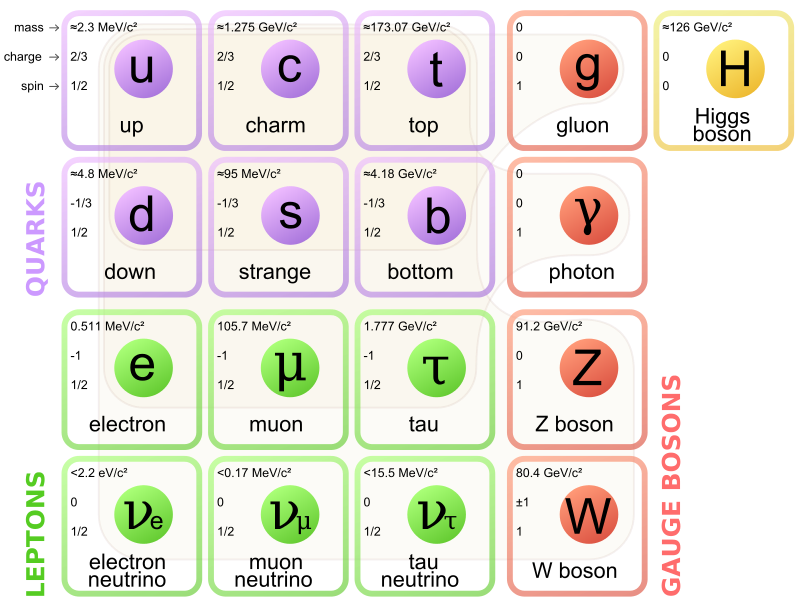
\includegraphics[width=0.8\linewidth]{Figures/chapter1_Figure/Standard_Model_of_Elementary_Particles.png}
\end{center}
\caption{The elementary particles given in three generations of matter, the gauge bosons in fourth column and the Higgs boson
in the fifth.}
\label{Fig:Standard_Model_of_Elementary_Particles}
\end{figure}

\begin{table}[!htbp]
\caption{Gauge bosons and their masses, coupling constants and interaction ranges for the three forces of the SM}
\begin{tabular}{|c|c|c|c|}
\hline
Force  &  Weak & Electromagnetic & Strong \\ \hline
Mediator boson & $W^{\pm}$ and $Z$ & photon ($\gamma$)& Gluon (g) \\ \hline
Mass(GeV)    & 80.4, 91.2 GeV& 0& 0 \\ \hline
Coupling Constant & $G_F\approx  1.2 \times 10^{-5}$~\ensuremath{\mathrm{GeV^{-2}}} & $\alpha=\frac{1}{137}$ & $\alpha_s\approx 0.1$  \\ \hline
Interaction Range &$10^{-16}$~cm& $\infty$& $10^{-13}$~cm \\ \hline
\end{tabular}
\end{table}
\subsection{Fundamental Interactions}\label{fundamentalforces}
The three fundamental interactions (electromagnetic, strong and weak) are explained three dedicated
theoretical descriptions Quantum Electrodynamics (QED), Quantum Chromodynamics (QCD) and  Quantum Flavourdynamics (QFD) which are 
encoded in SM. Electromagnetic and weak interactions were then unified into electroweak (EWK) interaction
%at the unification energy scale of the order of 100~GeV 
with significant contributions by Abdus Salam, Sheldon Glashow and Steven Weinberg. The mathematical 
description of interaction of charged particles are described by QED. Photon of QED is the force carrier of electromagnetic force. QED is the first theory which explains the interaction between light and matter that patches up special relativity and quantum mechanics. Figure \ref{Fig:Feynmann_Diagram_Gluon_Radiation}
shows an example of QED, electron-positron annihilation. Annihilation is the process of destruction of particle and anti particle pair to any set of particles 
obeying conservation of 
quantum numbers, energy and momentum. QED is perturbative theory based on fundamentals of quantum mechanics
established by three distinguished physicists W. Heisenberg, W. Pauli and P. A. M. Dirac during 1920s. Later on,  Freeman J. Dyson, Richard P. Feynman  and Julian S. Schwinger showed 
that
charged particle can possibly interact through a sequence of processes with growing complexity, and all of these processes could be 
described by Feynman developed  graphical technique. QED is abelian gauge theory with $U(1)$ being its symmetry group.
\begin{figure}
\begin{center}
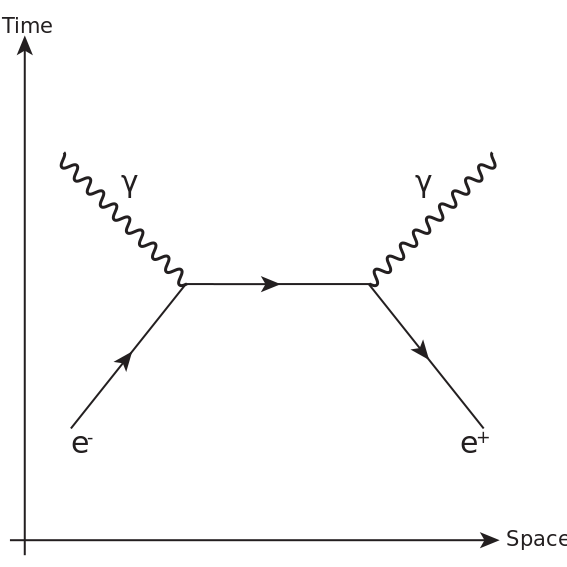
\includegraphics[width=0.5\linewidth]{Figures/chapter1_Figure/Annihilation_of_a_Positron_Electron_pair.png}
\end{center}
\caption{A Feynman diagram of annihilation of electron positron.}
\label{Fig:Feynmann_Diagram_Gluon_Radiation}
\end{figure}
\par Weak interaction, one of the four fundamental forces, was first revealed by the understanding of beta decay in 1933 by Enrico Fermi called Fermi's 
interaction~\cite{Referencea}. Weak force is mediated by $W^\pm$ and $Z$ bosons. In terms of a field theory, it is represented by gauge theory with symmetry group $SU(2)$, 
having three gauge bosons ($W^+, W^-, Z$). Weak force, rarely known from quantum flavordynamics (QFD), is the only force which is 
proficient to change the flavor of quarks. This is very short range force 
because exchange bosons ($W^\pm$, $Z$) are massive. All fermions and the Higgs boson can interact via weak force. In 1970s, electromagnetic and weak
forces were unified as electroweak force above unification energy (on the order of 100 GeV). The Physics Nobel Prize was awarded to Sheldon Glashow, 
Abdus Salam, and Steven Weinberg for their role in electroweak unification. In the field theory representation, Electroweak unification is settled under the gauge group
\sutwol$\otimes$\uoneg~. Experimental observation of existence of electroweak interaction was accomplished in two phases, the first was disclosure of existence of neutral current in scattering  of neutrino in 1973 by Gargamelle collaboration and then the discovery of $W$ and Z gauge bosons in proton-antiproton collisions by both the UA1 and the UA2 
collaborations in 1983~\cite{Reference2,Reference3,Reference4,Reference5}. 
\par The representation of SM is made by \suthreec$\otimes$\sutwol$\otimes$\uoneg~gauge symmetry. Where \uoneg~is representation of QED, \sutwol~ represents weak theory and 
\suthreec~ represents QCD. By the unification of electromagnetic and weak force represented by \sutwol$\otimes$\uoneg \\ gauge symmetry \cite{Reference6}, Glashow, Salam and Weinberg was
able to formulate the fields to account the $W^\pm$, $Z$~and $\gamma$~(A) boson in footings of the original basis fields $A^{\prime}$~and $B$~as expressed 
in equations \ref{eqn:wmass}, \ref{eqn:zmass} ~and \ref{eqn:Amass}. The spontaneous breaking of \sutwol$\otimes$\uoneg~gauge symmetry is primary reason for the generation of masses of the particles and separate electroweak (EW) interaction from electromagnetic (EM) and weak interactions. At higher 
energies($>100~GeV$), both weak and EM forces acts as similar style. Further details would be described in \ref{chapter1_sec2} section. 
\begin{equation}
W_{\mu}^{\pm} = \sqrt{\frac{1}{2}} (A_{\mu}^{1}\pm iA_{\mu}^{2}) \qquad~M_W = \frac{1}{2}g\mathrm{v}
\label{eqn:wmass}
\end{equation}
\begin{equation}
Z_{\mu}^{\pm} = \sqrt{\frac{1}{g^{2}+g^{\prime2}}} (gA_{\mu}^{3} - g^{\prime}B_{\mu}) \qquad~M_Z = \frac{1}{2}\mathrm{v}\sqrt{g^2+g^{\prime2}}
\label{eqn:zmass}
\end{equation}
\begin{equation}
A_{\gamma} = \sqrt{\frac{1}{g^{2}+g^{\prime2}}} (gA_{\mu}^{3} - g^{\prime}B_{\mu}) \qquad~M_A = 0.
\label{eqn:Amass}
\end{equation}
\par One of the the four fundamental forces is the strong force which is responsible for strong nuclear force which bounds the nucleus of an atom. As the name speaks 
for itself, strong force is strongest among four fundamental forces, although it act at a distance of $10^{-15}$ meter (femtometer) or less. Strong force 
is described by QCD and only exist between quarks and gluons which carry non-vanishing color charges. In the field theory representation of the SM,
the strong force is represented by the symmetry group of \suthreec~. Here, C represents QCD color, which must be conserved in all such interactions. 
The strong interaction is mediated by gluons and contrary to the other fundamental forces, strong force does not diminish with gain in distance between quarks 
know as color confinement. As an implication of this property, no signature of elementary quark or gluon particle are observed 
in High Energy Physics (HEP) colliders, instead they bound with each other to form streams of hadrons by phenomenon known as hadronization called jets. 

%----------------------------------------------------------------------------------------
\section{The Brout-Englert-Higgs Mechanism (BEH)}\label{chapter1_sec2}
Gauge fields must acquire mass in order to correctly describe weak interaction and to be consistent with experimental findings. Before electroweak symmetry breaking (EWSB), 
all particles were supposed not to have masses, however mass term in electroweak Lagrangian for a gauge boson must be introduced to guarantee the 
renormalization of theory that would violate gauge invariance. Which hints that  some basic thing is missing in the theory apart from fermions and gauge
boson fundamental fields, which can maintain the local gauge invariance. The Higgs mechanism was postulated as a part of SM, which introduces the 
existence of a new scalar Higgs field. This field transformation ensures the renormalizability of the theory and gauge invariance. 
By this formulation
the concept of breaking of symmetry and origin of masses of the fermions and bosons ($W^{\pm}, Z$ boson) are introduced~\cite{Reference7,Reference8,Reference9,Reference10,Reference11,Reference12}. 
The Higgs mechanism introduces a doublet (under isospin) of complex scalar field 
\begin{equation}
\phi=\left(
  \begin{array}{c}
   \phi^{\dag}   \\
   \phi^{0} 
  \end{array}
\right)
=\frac{1}{\sqrt{2}}
\left(
  \begin{array}{c}
   \phi^{1}+i\phi^2   \\
   \phi^{3}+i\phi^4
  \end{array}
\right)
\label{eq:higgs_doublet_field}
\end{equation}
which can be substituted in electroweak lagrangian given below
\begin{equation}
 \mathscr{L}_{EWSB} = (D_{\mu}\phi)^{\dag}(D_{\mu}\phi)+\mathrm{V}(\phi^{\dag}\phi)
 \label{eq:EWSB_lagrangian}
\end{equation}
here $D_{\mu} = \delta_{\mu} - i gt_{a}W^{a}_{\mu}+\frac{i}{2}g^{\prime}YB_{\mu}$~represents covariant derivative and the lagrangian described in Equation 
\ref{eq:EWSB_lagrangian} is gauge invariant under the ~\sutwol$\otimes$~\uoneg~transformation. The kinetic energy term in the lagrangian is written 
in terms of the covariant derivatives whereas the potential only depends upon the product $\phi^{\dag}\phi$. $\phi$ is the scalar field and can be codified in terms of quantum numbers which are isospin ($I_3$), hypercharge (Y) and electric charge (Q):
%listed in Table~\ref{quantum_numbers}.
% \begin{table}[h!]
 \begin{center}
 \begin{tabular}{cccc}
   \hline\hline
  & $I_{3}$ & Y & Q  \\ \hline
  $\left(\begin{array}{c}\phi^{\dag} \\ \phi^{0} \end{array}\right)$ &$\left(\begin{array}{c}\frac{1}{2} \\ \frac{1}{-2} \end{array}\right)$ & $\left(\begin{array}{c} 1 \\ 1 \end{array}\right)$ & $\left(\begin{array}{c} 1 \\ 0 \end{array}\right)$\\   
  \hline
  \label{quantum_numbers}
 \end{tabular}
  \end{center} 
%  \end{table}
while the potential term in Equation ~\ref{eq:EWSB_lagrangian} can also be expressed as 
\begin{equation}
 \mathrm{V}(\phi^{\dag}\phi) = -\mu^{2}\phi^{\dag} \phi-\lambda(\phi^{\dag}\phi)^{2}
 \label{eq:higgs_potential}
\end{equation}
here $\mu$ is mass term and the parameter $\lambda$ represents the strength of the interaction. In the scenario, $ \mu > 0$ and $\lambda>0$ and the 
potential shapes becomes very interesting, which is essential for Higgs mechanism shown in Figure \ref{Fig:higgs_potential}. There occurs a minima for 
\begin{equation}
 \phi^{\dag}\phi =  \frac{1}{2}(\phi_{1}^{\dag}+\phi_{2}^{\dag}+\phi_{3}^{\dag}+\phi_{4}^{\dag}) =  \frac{-\mu^{2}}{2\lambda} \equiv \frac{\mathrm{V^{2}}}{2}
\end{equation}
but on the circle of points where the magnitude of z is $\phi$.
\begin{figure}
\begin{center}

\includegraphics[width=0.6\linewidth]{Figures/chapter1_Figure/higgs_potential}
\end{center}
\caption{The Higgs potential as in Eq.\ref{eq:higgs_potential}}
\label{Fig:higgs_potential}
\end{figure}
This minimum does not exist at a single value of $\phi$, but at circular non-zero values.The ($\phi^{\dag}\phi^0$) selection that affiliated with 
the ground state is arbitrary and in ($\phi^{\dag}\phi^0$) plane the selected point is not invariant under rotations which is called spontaneous symmetry breaking. To settle the ground state on the $\phi^0$ axis, the vacuum expectation value (VEV) of field $\phi$ is
\begin{equation}
 \langle\phi\rangle = \frac{1}{\sqrt{2}}=
 \left(
  \begin{array}{c}
   0   \\
   \mathrm{V}
  \end{array}
\right), \qquad \mathrm{V^2}=-\frac{\mu^2}{\lambda}.
\end{equation}
The field $\phi$ given below, is derived by rewriting it in some generic gauge, on footings of its VEV:
\begin{equation}
 \phi = \frac{1}{\sqrt{2}}e^{\frac{i}{\nu}\phi^{a}t_{a}\phi}=
  \left(
  \begin{array}{c}
   0   \\
   H+\nu
  \end{array}
\right), a=1, 2, 3
\end{equation}
here $\phi_a$ and $\phi_4 = H+\nu$ represents massless fields called Goldstone fields. New degrees of freedom is introduced
along with six degrees because of polarizations vector bosons $W^\pm$ and $Z$, as they are massless and scalar. A unitary gauge 
transformation in the field is fixed by
$$\phi^{\prime} =  e^{-\frac{i}{\nu}\phi^{a}t_{a}}\phi = \frac{1}{\sqrt{2}}
\left(
  \begin{array}{c}
   0   \\
   H+\nu
  \end{array}
\right)
= \frac{1}{\sqrt{2}}
  \left(
  \begin{array}{c}
   0   \\
   \phi^4
  \end{array}
\right) $$
so here we have zero expectation value for the Higgs field. \\
%Now if we rewrite the lagrangian in Eq.~\ref{eq:EWSB_lagrangian}~with field $\phi$ in unitary gauge, $\mathscr{L}_{EWSB}$ can be disintegrated
Now the lagrangian in Eq.~\ref{eq:EWSB_lagrangian}~ can be rewritten and disintegrated
into three components
\begin{equation}
 \mathscr{L}_{EWSB} = \mathscr{L}_{H}+\mathscr{L}_{HW}+\mathscr{L}_{HZ}
\end{equation}
where three terms is given, assuming approximation $\mathrm{V}=\mu^{2}H^{2}+\cos{t}$ and ignoring higher order terms:
\begin{align}
\mathscr{L}_{H} & = \frac{1}{2}\delta_{a}H\delta^{a}H+\mu^{2}H^{2}  \nonumber \\
\mathscr{L}_{HW } & = \frac{1}{4}\nu^{2}g^{2}W_{a}W^{\dag a}+\frac{1}{2}HW_{a}W^{\dag a} \label{Eq:modfied_langragian_HW}  \\
& = m_W^{2}W_{a}W^{\dag a}+g_{HW}W_{a}W^{\dag a}  \nonumber \\
\mathscr{L}_{HZ} & = \frac{1}{8}\nu^{2}(g^{2}+g^{\prime2})Z_{a}Z^{a}+\frac{1}{4}\nu(g^{2}+g^{\prime2})HZ_{a}Z^{a} \label{Eq:modfied_langragian_HZ} \\
& = \frac{1}{2}m_{Z}^{2}Z_{a}Z^{a}+\frac{1}{2}g_{HZ}HZ_{a}Z^{a}.  \nonumber 
\end{align}
%
For $W^{\pm}$ and $Z$ bosons, mass terms are included in Eqs.~\ref{Eq:modfied_langragian_HW}~and~\ref{Eq:modfied_langragian_HZ}. This adds up three additional degree of freedom; however, three of the total four Goldstone bosons have also been vanished from the Lagrangian $\mathscr{L}_{EWSB}$ not affecting overall number of degrees of freedom. A new scalar field has been introduced referred as Higgs field, introduced in the theory. The boson associated
of Higgs field.
%rephrase
\\ Briefly, the BEH mechanism ensures the renormalizability of theory and explain existence of the massive weak gauge bosons, despite of the fact that 
the fundamental gauge boson in theory still stays to be massless. In fact, the symmetry still exist in equation so using ``hidden`` is preferred over broken.   
According to BEH mechanism, fermions also acquire masses via their interaction with Higgs field. The invariance of the Higgs field minimum for \uoneg~group shows that the electromagnetic symmetry is not broken spontaneously that keeps photon massless.
%\subsection{Vector Boson Masses and Couplings}
\subsection{Masses and Couplings of Vector Bosons}
Equations. \ref{Eq:modfied_langragian_HW} and \ref{Eq:modfied_langragian_HZ} show that masses of $W^{\pm}$ and $Z$ bosons are associated with coupling constants of electroweak and a parameter $\nu$ which is
VEV that defines a mass scale property of EWSB:
\begin{equation}
  \begin{cases}
    m_W = \frac{1}{2}\nu g \\
    m_Z = \frac{1}{2} \sqrt{g^2+g^{\prime 2}} \\
  \end{cases}
\rightarrow
\frac{m_W}{m_Z} = \frac{g}{\sqrt{g^2+g^{\prime 2}}} = \cos (\theta_W).
\end{equation}
Couplings of Higgs boson to the bosons can also be obtained by Eqs. \ref{Eq:modfied_langragian_HW} and \ref{Eq:modfied_langragian_HZ}
\begin{equation}
g_{HW} = \frac{1}{2} \nu g^{2} = \frac{2}{\nu}m_{W}^{2}
\label{Eq:coupling_HW}
\end{equation}
\begin{equation}
g_{HZ} = \frac{1}{2} \nu (g^2+g^{\prime 2}) = \frac{2}{\nu}m_{Z}^{2}.
\label{Eq:coupling_HZ}
\end{equation}
Using above Eqs. \ref{Eq:coupling_HW} and \ref{Eq:coupling_HW} helps to get the ratio of Higgs decay to $W^{\pm}$~and~$Z$ bosons
\begin{equation}
\frac{\mathcal{B}(H\rightarrow W^+ W^-)}{\mathcal{B}(H\rightarrow Z Z)} = \left( \frac{g_{HW}}{\frac{1}{2}g_{HZ}}^{2}\right) = 
4\left(\frac{m_W^2}{m_Z^2}\right)^4 \approx 2.4.  
\end{equation}
At last, the characteristic mass scale for EWSB may be obtained by the relation between the Fermi constant $G_F$ and 
the $\nu$ parameter:
\begin{equation}
 \nu = \left(\frac{1}{\sqrt{2}G_F}\right) \approx 246 GeV.
\end{equation}

\subsection{Fermions Masses and Couplings}
Fermions couples to Higgs  field to acquire mass by Higgs mechanism. This can be achieved by introducing an invariant term \sutwol~$\times$~\uoneg~
(which is called yukawa term) in SM lagrangian which can describe interactions between Higgs and the fermion fields. $\phi$ is an iso-doublet and the fermions
can be split into right-handed and left-handed singlet. So, the yukawa term for each fermion will have expression given below for leptons:
\begin{equation}
 \mathscr{L}_{\ell} =  -G_{\ell}.\bar{l_\ell}\phi\ell{R}+\bar{\ell_R}\phi^{\dag}l_{\ell}.
\end{equation}
A mass term will only evolve for second component of $l_\ell$ because first part of $\phi$ is zero. Actually, this also depicts that the neutrinos are massless.

\begin{equation}
\mathscr{L}_{\ell} = -\frac{G_{H\ell}}{\sqrt{2}}\nu\bar{\ell}\ell-\frac{G_{H\ell}}{\sqrt{2}}H\ell\bar{\ell}. 
\label{Eq:leptons_yukawa_lagrangian}
\end{equation}
For quarks, down type quarks(i.e. down, strange and bottom) behave similar to the leptons while up type quarks (i.e. up , charm, top) should couple to the charge conjugate of $\phi$
\begin{equation}
 \phi_c =  -i \tau_2 \phi^{*} = \frac{1}{\sqrt{2}}\left(
   \begin{array}{c}
   \phi^{3}+i\phi^4   \\
   -\phi^{1}+i\phi^4
  \end{array}
 \right)
\end{equation}
in unitary gauge that becomes
\begin{equation}
 \phi_c=
 \frac{1}{\sqrt{2}}\left(
   \begin{array}{c}
   \eta+\nu \\
    0
  \end{array}
 \right).
\end{equation}
Therefore, the yukawa Lagrangian can be expressed as 
\begin{equation}
 \mathscr{L} = -G_{H\ell}\bar{L_L}\phi\ell_{R}-G_{Hd}\bar{Q_L}\phi d_R-G_{Hu}\bar{Q_L}\phi^{c}u_R+h.c.. 
\end{equation}
The couplings constant and mass of a fermion can be derived from Eq. \ref{Eq:leptons_yukawa_lagrangian}, written as
\begin{equation}
m_f = \frac{G_{Hf}}{\sqrt{2}}\nu
\end{equation}
\begin{equation}
 g_{Hf} = \sqrt{G_{Hf}}{\sqrt{2}}=\frac{m_f}{\nu}.
\label{Eq:fermions_couplings}
\end{equation}
The fermions mass can not be predicted by the theory as $G_{Hf}$ is free parameters. 
An fermion object acquires mass when Higgs field interacts with it to trans the right-handed chirality into the left-handed chirality and vice versa. 
%The interaction of Higgs field with fermions
%transforms right-handed chirality in a left-handed chirality and vice versa in a way that object acquire mass. 
The strength of the interaction of Higgs fields with particles is  reflected by its mass.
\par This evaluation is rather interpretative, as it not accumulating the fact of  
three families of leptons and quarks in reality.
%there are three families of quarks and leptons in reality.
The difference between eigenstates of weak mass and the eigenstates of physical mass makes real analysis complicated.
Transformation of the weak mass basis to physical basis  in essential to deal with the physical particles.
For quark sector, it is achieved by Cabibbo-Kobayashi-Maskawa (CKM) matrices and in case of lepton sector, it is done by Pontecorvo-Maki-Nakagawa-Sakata (PMNS) matrices.
%This is achieved by the usual unitary transformation matrices, Cabibbo-Kobayashi-Maskawa (CKM) and Pontecorvo-Maki-Nakagawa-Sakata (PMNS) matrices, for quark and lepton sectors respectively.
%----------------------------------------------------------------------------------------
%\section{Production and Decay of the Higgs Boson }\label{chapter1_sec3}
\section{Higgs boson Production and its Decay }\label{chapter1_sec3}
After electroweak unification, spontaneous symmetry breaking and addition of Higgs mechanism to SM solved all the puzzles with an assumption that there exists the Higgs boson. This boson was considered as the last missing subject of the SM and has been searched at LHC within full mass range allowed i.e from 114~GeV to 1~TeV (given unitary and above LEP constraints). 
Discussing the production and decay modes of Higgs would allow us to point out the most suitable decay channels Higgs boson discovery point of view and its properties measurements. Theory does not predict the
Higgs mass; however, its couplings with bosons are proportional to the square of their  masses as shown in Eqs.~\ref{Eq:coupling_HW}~and~\ref{Eq:coupling_HZ}. In case of 
fermions, there is direct proportionality between their couplings with the Higgs and their masses as in Eq.~\ref{Eq:fermions_couplings}. For this reason, the
most promising channels for Higgs searches are its decays to $W^+W^-$, $ZZ$ and third generation of leptons. 
Also, photon being massless particle does not couple to Higgs directly but through loop contributions (most probable are top quark and $W^\pm$ boson loops). 

\subsection{Higgs boson Production}\label{chapter1_sec4}
The production modes of Higgs which are dominant in proton proton collisions at LHC are illustrated in Figure~\ref{Fig:Higgs_boson_production_at_LHC},
corresponding production cross sections as a function of its mass at center-of-mass energies i.e. $\sqrt{s} =$~7, 8 and 13 TeV are shown in
Figure~\ref{Fig:Higgs_boson production_crossSection_at_LHC}. A considerable increase in production cross section of Higgs is found as we move towards higher center-of-mass energies (Figure~\ref{Fig:Higgs_boson_production_at_LHC_sqrt}~\cite{Referenceb}).
\begin{figure}
\begin{center}
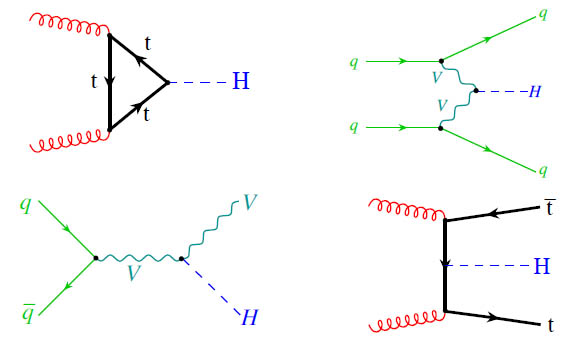
\includegraphics[width=0.7\linewidth]{Figures/chapter1_Figure/HiggsProduction.jpg}
\end{center}
\caption{Feynman diagrams of Higgs production at tree level: gluon-gluon fusion (upper left);VV fusion (upper right);
associated production with W and Z bosons (bottom left); associated production with $t\bar{t}$ (bottom right). }
\label{Fig:Higgs_boson_production_at_LHC}
\end{figure}
\begin{figure}
 \begin{center}

\includegraphics[width=0.6\linewidth]{Figures/chapter1_Figure/Higgs_XS_7TeV.pdf}
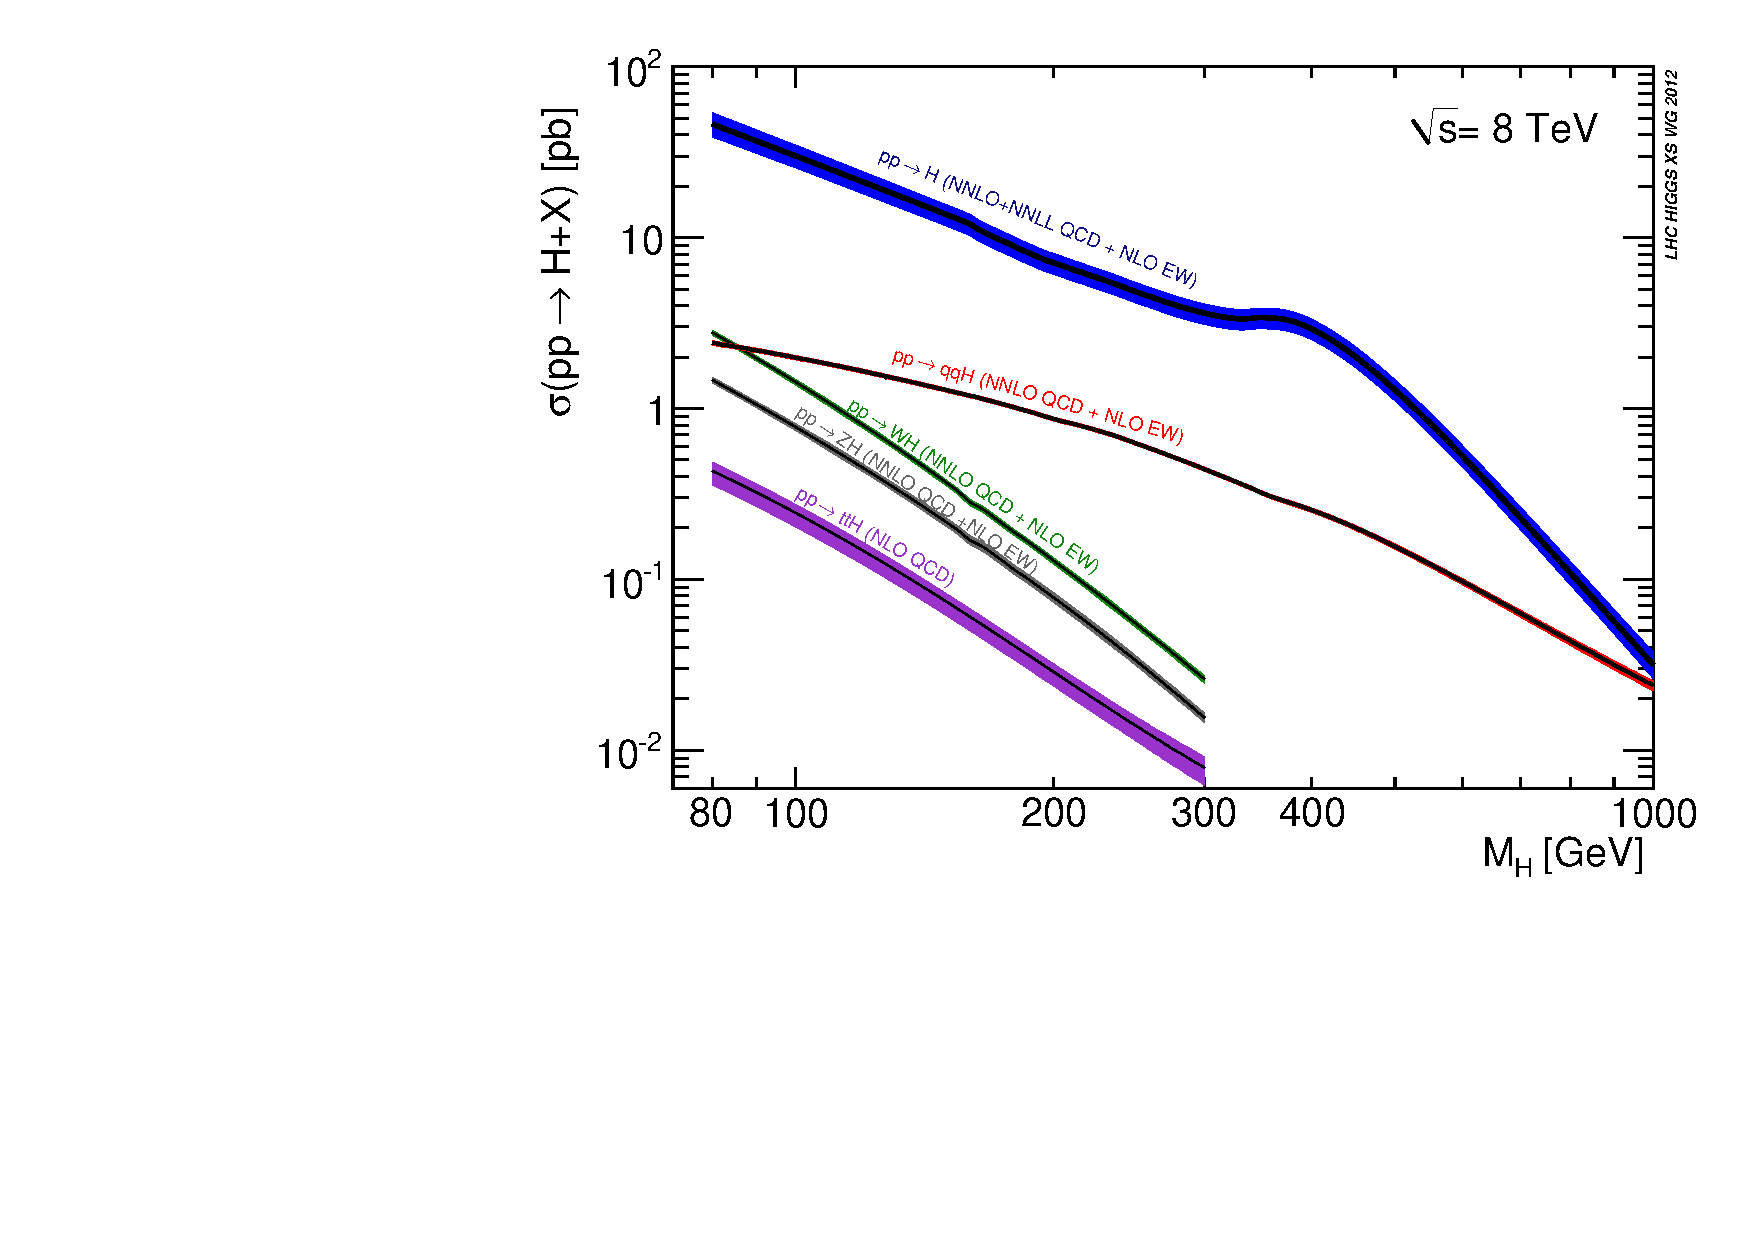
\includegraphics[width=0.6\linewidth]{Figures/chapter1_Figure/Higgs_XS_8TeV.pdf}
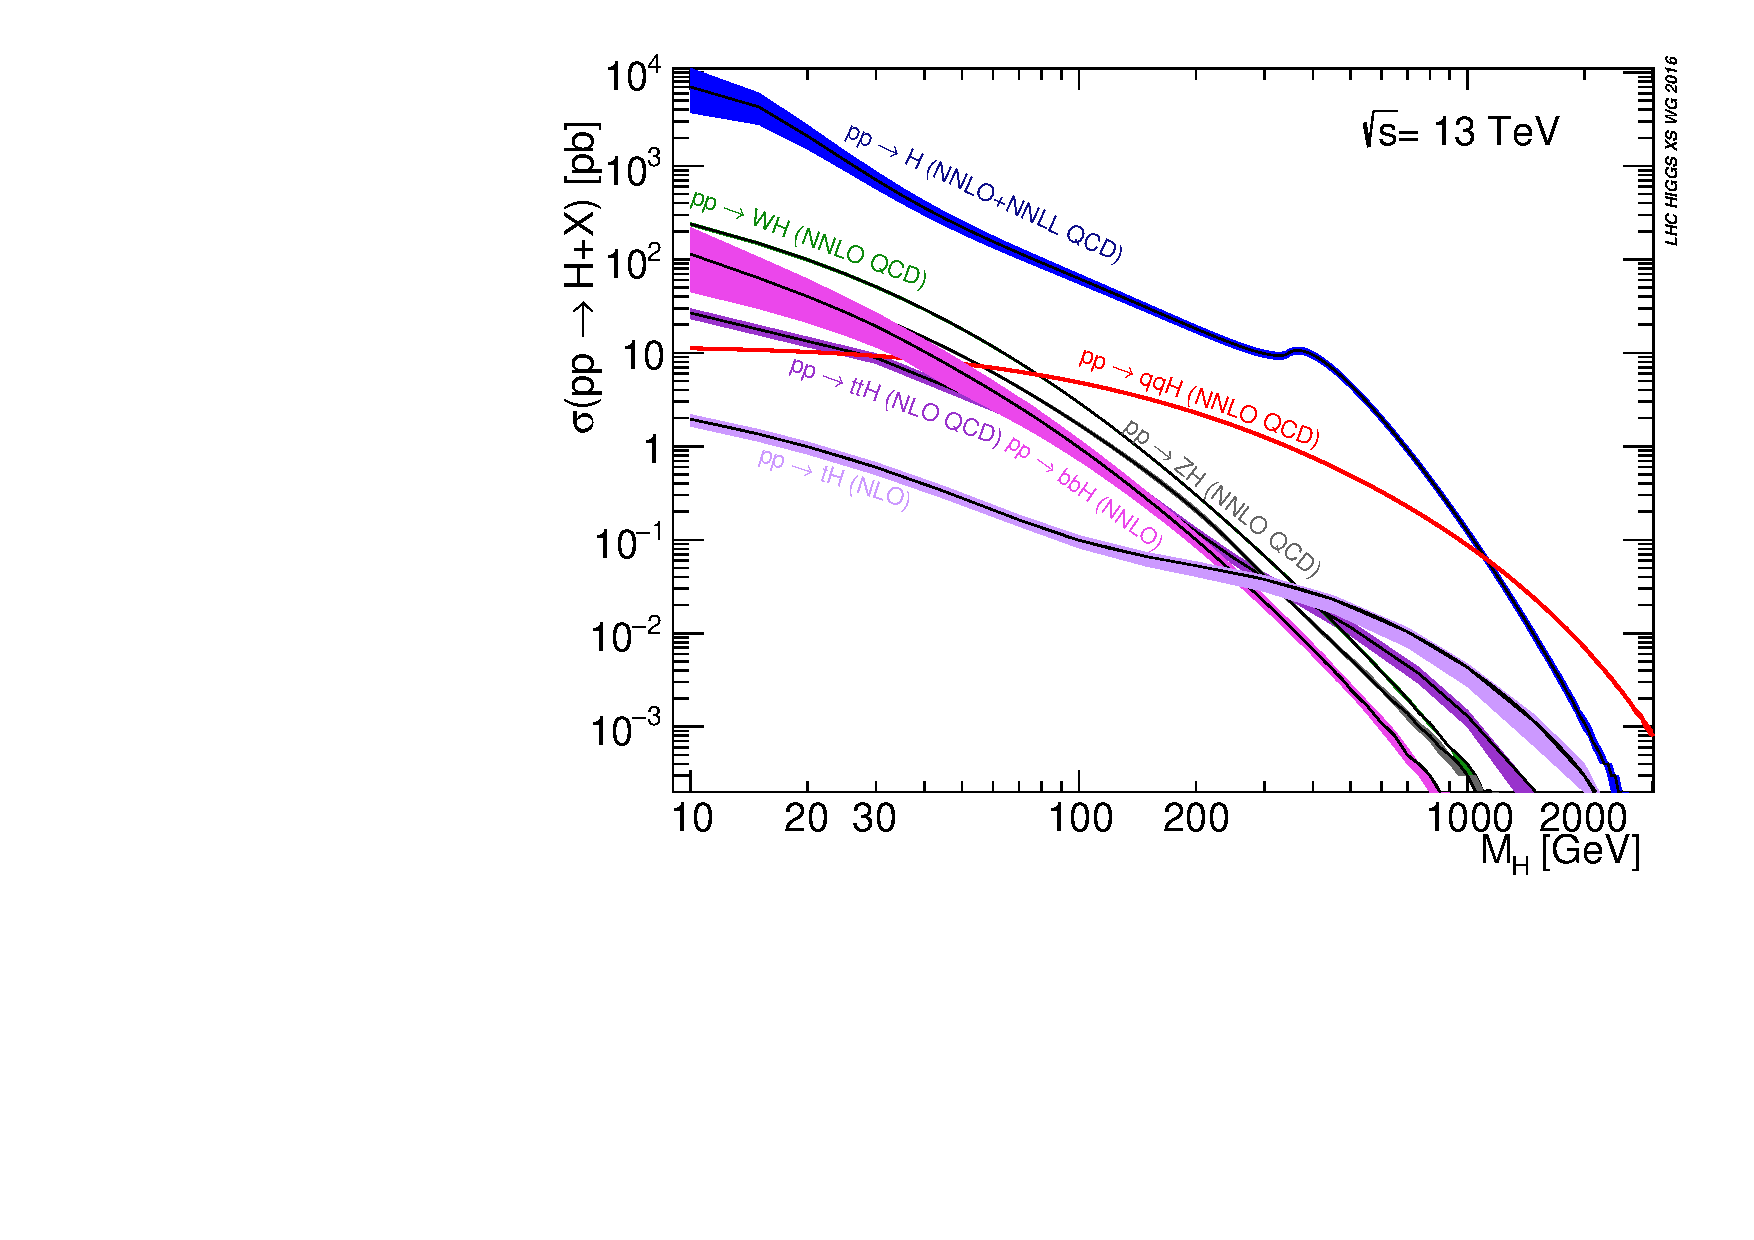
\includegraphics[width=0.6\linewidth]{Figures/chapter1_Figure/plot_13tev_BSM_aa.pdf}
\end{center}
\caption{Production cross sections of SM Higgs boson at 7, 8 and 13 TeV as function of its mass.}
\label{Fig:Higgs_boson production_crossSection_at_LHC}
\end{figure}
\begin{figure}
 \begin{center}
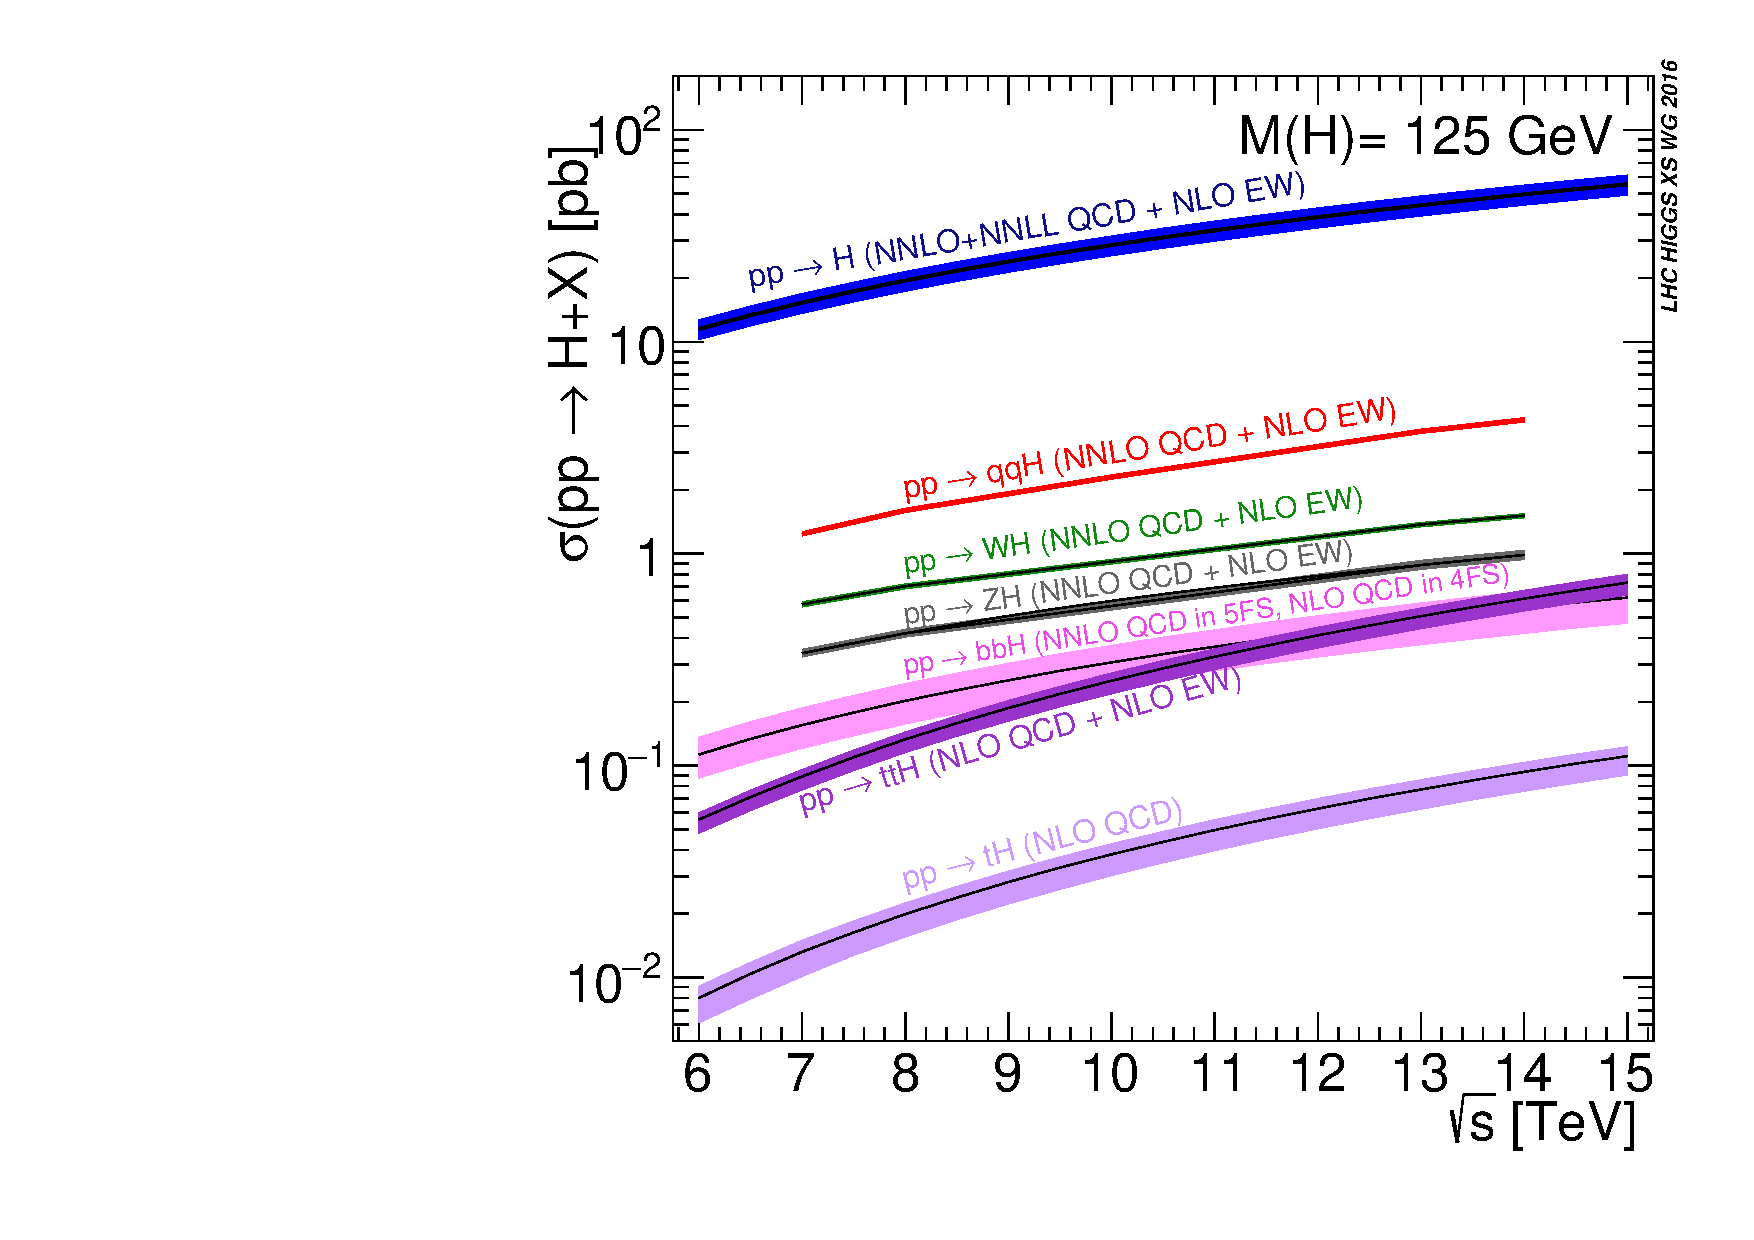
\includegraphics[width=0.6\linewidth]{Figures/chapter1_Figure/Escan_h125.pdf}
\end{center}
	\caption{Production cross sections of Higgs boson ($m_H =125$~GeV)  as a function of center of mass energies}
\label{Fig:Higgs_boson_production_at_LHC_sqrt}
\end{figure}
\subsubsection{Gluon-gluon Fusion }
The most dominant production mode of Higgs at LHC is gluon-gluon fusion as illustrated in 
%mode in whole mass range and center-of-mass energies range is gluon-gluon fusion ($\ggH$), illustrated in 
Figure~\ref{Fig:Higgs_boson_production_at_LHC}~(top left)~\cite{Referenceb}. As
LHC and tevatron are hadron colliders, it highly probable that two gluons responsible for binding of hadron collide. The gluons couples to Higgs through the loop of virtual 
quarks, as coupling is directly proportional to fermion mass, top quark loop is most dominant. For SMHiggs ($m_H = 125$~GeV) the ggH cross section at 7~TeV, 8~TeV and 13~TeV are approximately 15, 19, 44~pb respectively. As we move towards higher
energies the production cross section increases significantly, i.e 27\% from
7~TeV to 8~TeV and ~227\% from 8~TeV to 13~TeV at $m_H = 125$~GeV. The cross section numbers in Table~\ref{Tab:higgs_cross_Section_ggH_vbf} are evaluated at NNLO (QCD) and NLO (EW) accuracies.
\subsubsection{Vector Boson Fusion (VBF)}
VBF is second most important production mode of Higgs at LHC and LEP as shown in 
Figure~\ref{Fig:Higgs_boson_production_at_LHC}~(upper right). Its cross section is roughly 10~times lower than ggH at
$m_H = 125$~GeV, and becomes comparable at $m_H = 1$~TeV. For SM Higgs at $m_H = 125$~GeV %center-of-mass energies 
its cross section at 7~TeV, 8~TeV and 13~TeV are approximately 1.2, 1.6, 3.8~pb respectively. The cross section numbers in the Table~\ref{Tab:higgs_cross_Section_ggH_vbf} are
computed at NNLL QCD and NLO EW precision~\cite{Referenceb}. In VBF production mode, two $W^\pm$ or $Z$ boson fusion create 
Higgs that have been emitted by a (anti)fermion pair collision. The VBF experimental signal is very clean and can be well distinguished from ggH with
two high energy jets in detected in forward region. These jets signature helps to increase signal to background ratio. 

\begin{table}
\caption{Higgs boson production cross sections in pb for different Higgs masses and center-of-mass energies by ggH and VBF productions mechanism at LHC.}
 \begin{center}
 \begin{tabular}{|c|ccc|ccc|}
  \hline
  $m_H(GeV)$&&ggH&&VBF&& \\ \hline
  &7~TeV&8~TeV&13~TeV&7~TeV&8~TeV&13~TeV \\ \hline
  $120$&16.61&21.07&47.38&1.30&1.68&3.9 \\
  $125$&15.31&19.47&44.14&1.24&1.60&3.78 \\
  $130$&14.15&18.03&41.23&1.19&1.53&3.64 \\
  \hline
 \end{tabular}
 \end{center}
 \label{Tab:higgs_cross_Section_ggH_vbf}
\end{table}
%rephrase 2pm
\subsubsection{Production of Higgs in association with W and Z bosons}
Such production of Higgs is known as Higgs Strahlung as illustrated in 
Figure~\ref{Fig:Higgs_boson_production_at_LHC}~(bottom left). In this process, 
Higgs is radiated by high energetic $W^\pm$ or $Z$ bosons that is produced by fusion of two fermions. This production mode was leading mechanism at LEP and sub-leading mechanism at Tevatron. At LEP it becomes very probable to produce $W^\pm$ or $Z$ boson with electron positron collisions. In case
of hadron collider,  tevatron makes quark antiquark collisions more likely as compared to LHC. AT LHC this production mechanism is at third number. The 
WH and ZH cross section for Standard Model Higgs  at center-of-mass energies of 7~TeV, 8~TeV and 13~TeV are listed in 
Table~\ref{Tab:higgs_cross_Section_WH_ZH_ttH} which are computed at NNLL QCD and NLO EW precision~\cite{Referenceb}. 
\subsubsection{Top Fusion}
The least dominant process of Higgs production is illustrated in Figure~\ref{Fig:Higgs_boson_production_at_LHC}~(bottom right). In this process two gluons
collide producing pair of top antitop which produces Higgs by fusion in association $t\bar{t}$. The ttH cross section for Standard Model Higgs  at center 
of mass energies  of 7~TeV, 8~TeV and 13~TeV are listed in Table~\ref{Tab:higgs_cross_Section_WH_ZH_ttH} which are computed at  NLO QCD and NLO EW 
precision~\cite{Referenceb}. 
\begin{table}
\caption{Higgs boson production cross section in pb for different Higgs masses and center-of-mass energies  by associative productions mechanism at  LHC.}
 \begin{tabular}{|c|ccc|ccc|ccc|}
  \hline
  $m_H(GeV)$&&WH&&&ZH&&&ttH& \\ \hline
  &7~TeV&8~TeV&13~TeV&7~TeV&8~TeV&13~TeV&7~TeV&8~TeV&13~TeV \\ \hline
  $120$&0.66&0.81&1.57&0.39&0.48&0.99&0.11&0.15&0.57 \\
  $125$&0.58&0.70&1.37&0.34&0.42&0.88&0.09&0.13&0.51 \\
  $130$&0.51&0.62&1.21&0.30&0.37&0.79&0.08&0.12&0.45 \\ \hline
 \end{tabular}
 \label{Tab:higgs_cross_Section_WH_ZH_ttH}
\end{table}
%gluon-gluon fusion (top left); 
%VV fusion (top right); W and Z associated production (bottom left); t\bar{t} associated production (bottom right).

\subsection{Higgs Decay}
As Higgs boson is electroweak particle, so it wants to decay quickly. 
Likelihood of its decay depends on many aspects, i.e. its mass, interaction strength and etc. Most of the factors are controlled by SM except the Higgs boson mass itself.
%The Higgs boson decay likelihood depends on a variety of aspects, i.e mass of the 
%Higgs boson, interaction strength etc, most of these factors are controlled by SM except the Higgs boson mass itself. 
%rephrase, night 19.06.2020
The life time of SM 126 GeV Higgs is $1.6\times10^{-22}$~s. It can decay to all SM particles with mass but it likes to decay most 
heavier particles available. Higgs boson decay branching ratio to a variety of particles are illustrated in Figure~\ref{Fig:Higgs_BR}~\cite{Referenceb}.
\par $H\rightarrow b\bar{b}$ (at $m_H \approx 125$~GeV) is the most dominant decay mode of Higgs. But the QCD background in this channel is of
many order higher than signal which makes it less sensitive channel. 
However, CMS and ATLAS collaborations and other collaborations ~\cite{Reference13}, ~\cite{Reference14} and ~\cite{Reference15}(CDF and D0) have exploited this channel, in association with a vector boson which decays to leptons, in boosted regime. B quarks are also difficult to reconstruct in a detector. When they decay in the detector, they fragment into jets of many hadrons. These jets are difficult to  
reconstruct perfectly. Because of this, it is necessary to exploit other channels in this region. $H \rightarrow \gamma\gamma$ is one most favorable decay channel due 
to signature with two high energy photons with excellent mass resolution. 

The main backgrounds in this channel are $q\bar{q} \rightarrow \gamma\gamma$, $\Pg\Pg \rightarrow \gamma\gamma$ and instrumental background where one or two jets are misidentified to be photons. 
As the Higgs mass at 125~GeV, Higgs boson decay to diboson($WW, ZZ$) boson are also available, where one or both boson can be off-shell. In case of $WW$ decay, its 
impossible to completely reconstruct $WW$ boson in detector as it decays $H \rightarrow WW \rightarrow \ell\nu\ell\nu$ have two neutrinos and
$H \rightarrow WW \rightarrow \ell\nu jj$ have one neutrino and two jets. These objects pulls mass distribution to be wide and signal to background ratio 
to be low, which makes $WW$ decay channel less sensitive. While $H \rightarrow ZZ \rightarrow \ell\ell\ell\ell$ decay is labeled as golden channel in 
spite of low branching ratio. The clean signature of at least four leptons makes this channel almost background free. These leptons are high energetic 
leptons which can reconstructed with excellence in the detector. The branching ratio of the Higgs in intermediate range is illustrated in 
Figure~\ref{Fig:XSBR_7TeV_8TeV_SM_LM}~\cite{Referenceb}.
 \begin{figure}
 \begin{center}

\includegraphics[width=0.6\linewidth]{Figures/chapter1_Figure/Higgs_BR_LM.pdf}
%
\includegraphics[width=0.6\linewidth]{Figures/chapter1_Figure/Higgs_BR.pdf}
\end{center}
\caption{Branching ratios for different Higgs  boson decay channels as a function of the Higgs mass.}
\label{Fig:Higgs_BR}
\end{figure}
\begin{figure}[!htbp]
\begin{minipage}{0.5\linewidth}
\centerline{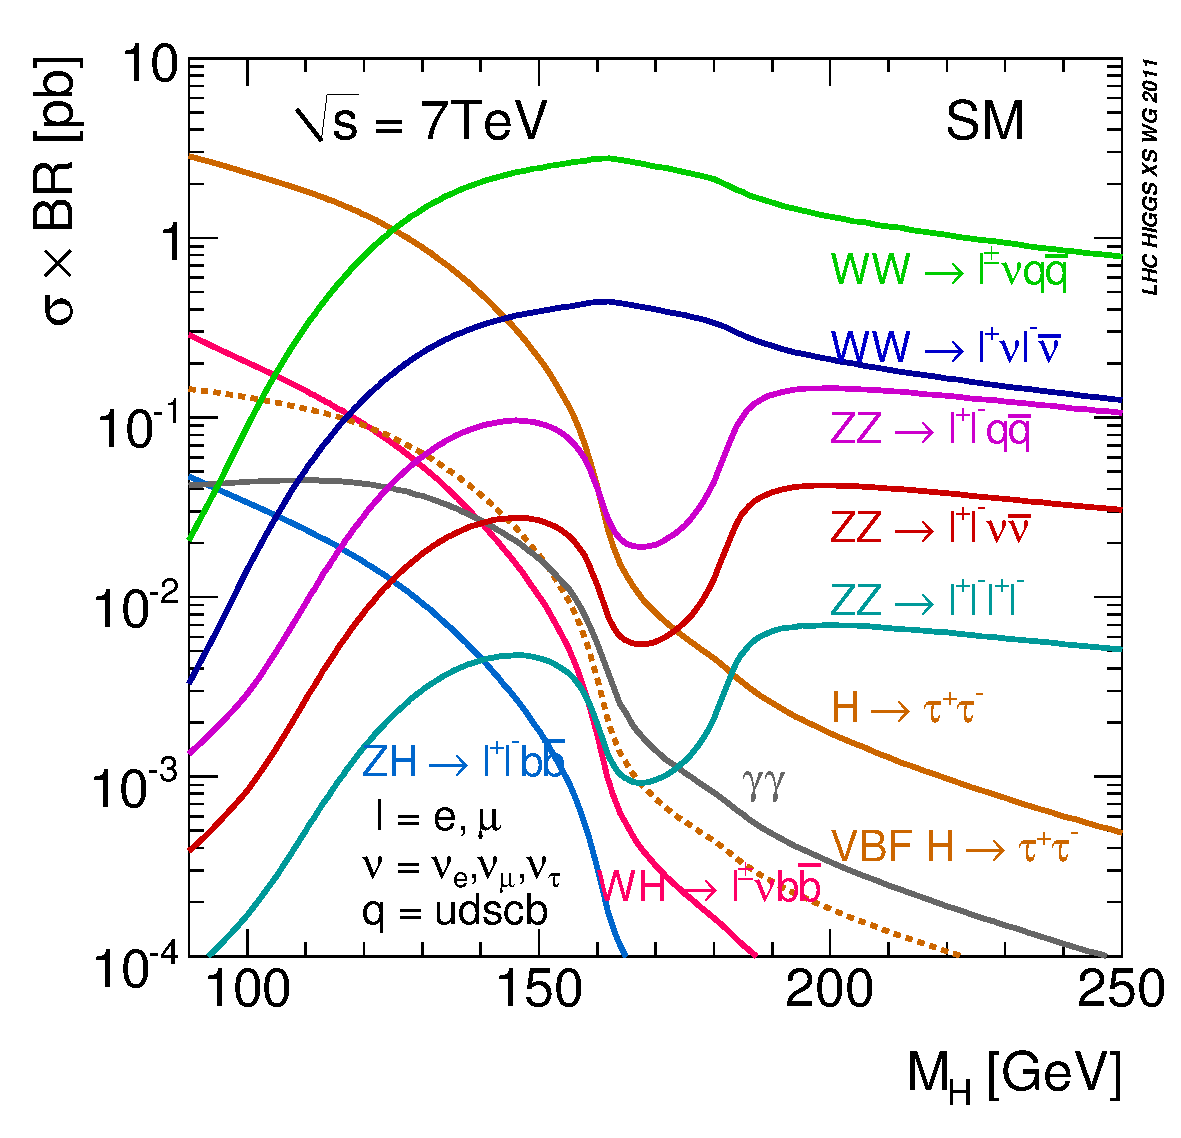
\includegraphics [width=\linewidth] {Figures/chapter1_Figure/XSBR_7TeV_SM_LM.pdf}}
\end{minipage}
\begin{minipage}{0.5\linewidth}
\centerline{
\includegraphics [width=\linewidth] {Figures/chapter1_Figure/XSBR_8TeV_SM_LM.pdf}}
\end{minipage}
	\caption{Cross sections of Higgs times branching ratios at 7 TeV and 8 TeV (left and right diagrams respectively).}
\label{Fig:XSBR_7TeV_8TeV_SM_LM}
\end{figure}
%-----------------------------------------------------------------------------------------
\section{Experimental Observations}\label{chaper1_sec4}
 The electroweak unification theory lead to series of impressive experimental discoveries. In 1973, the evidence of
 neutral current through inelastic scattering was found by Gargemelle buddle chamber collaboration at CERN~\cite{Reference16}. This
 evidence provide
 starting platform to the Standard Model of electroweak interaction.
 \par Super Proton Synchrotron proton-atniproton collider at CERN played its role to next breakthrough that came a decade later. The existence
 of $W$, $Z$ boson
 announced by UA1 and UA2 collaboration through the channels
 $Z \rightarrow \mu^+ \mu^-$, $Z \rightarrow e^+ e^-$ and $ W \rightarrow e\nu$~\cite{Reference2,Reference3,Reference4,Reference5}. This was a first
 observation of $W, Z$ boson that mediates weak force. For their contributions, Simon van dar Meer and Carlo Rubbia were awarded with Nobel Prize for their contribution in 1984.
 \par These important experimental discoveries and growing knowledge on weak interaction convinced to construct the LEP collider.
 at
 CERN, for  deeper look into $W,Z$ further decays, their precise mass measurement~\cite{Reference17,Reference18}. LEP was equipped with four detectors around the ring; OPAL (Omni-Purpose Apparatus for LEP), DELPHI (Detector with Lepton and Hadron Identification), ALEPH(Apparatus for LEP Physics) 
  and L3 (Letter of Intent 3). These experiments reported 
 many precise results of the SM, specially masses of W and Z bosons and confirming three neutrino species consistent with Standard
 Model~\cite{Reference18}.
 \par Around 2000, construction for the Large Hadron Collider (LHC)~\cite{Reference19} at CERN was started to look for last missing patch of SM, the Higgs boson. LHC is equipped with four major detectors; ATLAS (A Toroidal LHC Apparatus), CMS (Compact Muon Solenoid), ALICE (A Large Ion Collider Experiment), LHCb (Large Hadron Collider beauty). 
 LHC had shown brilliant performance since being operational. It has already recorded data of proton-proton collisions at center-of-mass energies 7,8 and 13~TeV in from 2011 to 2018. After a long search , the CMS and ATLAS collaboration of LHC, certified the presence of the Higgs, a heavy scalar boson, on 4 July 2012~\cite{Reference20,Reference21}. Further test to measure 
 of the properties of this scalar boson immediately begins, in March 2013, CERN announced the tentative confirmation of consistency of its properties  with 
 SM~\cite{Reference22,Reference23,Reference24,Reference25}.
\section{Beyond Standard Model}\label{chapter1_sec5}
Although SM has passed numerous experimental test with great precision, it is not considered to be theory of everything. There are many 
phenomena which are not explained by SM i.e Hierarchy problem, lack of direct detection of dark matter and dark energy, and masses of neutrinos etc. There are several theoretical 
extension posed in Standard Model such as Minimal Super Symmetrical Model(MSSM) and Next-to-Minimal Super Symmetric Standard Model (NMSSM) or completely new 
theoretical description, such as string theory, extra dimension. The simplest broadening of Higgs sector of SM is the the electroweak singlet (EWS) model~\cite{Reference26}.
In this model, a heavy singlet is defined along with SM scalar Higgs field and then two CP-even Higgs bosons comes out as result of spontaneous symmetry 
breaking. 
 Another generic extension to SM Higgs sector is 2 Higgs Doublet Model (2HDM), which introduces two scalar, complex doublet $\phi_1$ 
 and $\phi_2$~\cite{Reference27}. Spontaneous symmetry breaking results five Higgs boson, a neutral CP-odd one (A), two charged ($\mathrm{H}^{\pm}$) and two CP-even particles (h and H). Experiments are looking for any direct or indirect hints of new physics. Some of main aspects where SM is unable to explain are discussed below.
\subsection{Hierarchy Problem}
 Larger discrepancy between features of the gravitational and the weak forces is known as  ``Hierarchy Problem''.
There does exist a convincing explanation of the problem why weak force is $10^{32}$ times stronger than gravitational force. The
field theory breaks down because of existence of quantum gravity at plank scale ($M_p \approx 10^{19}$~GeV).
Writing the Standard Model Lagrangian for the Higgs mass will lead to following expression below
\begin{equation}
 m^{2}_{H} = m^{2}_{oH} + \delta m^{2}_{H}
\end{equation}
here $m^{2}_{oH}$  represents  mass parameter exist in the Standard Model Lagrangian, and
 $\Delta m^{2}_{H}$ represents the quantum radiative corrections to the mass that are predicted to be heavier.
These corrections can be found as
\begin{equation}
 \Delta m^{2}_{H} \approx \frac{\lambda^2}{16\pi^2}\Lambda^2
\end{equation}
here $\lambda$ represents the Yukawa coupling constant, and $\Lambda$ represents the energy at
which the Standard Model is invalid, or about 1~TeV. This was also one of the reason to expect Higgs boson mass at order of few hundred GeV. The 
Super symmetry (SUSY)
provide the solution of Hierarchy problem by predicting the existence of heavier super partners of all SM particles (bosons and fermions). Several 
direct and
indirect searches has been conducted at LHC to hunt for SUSY, but no evidence has been found so far.
\subsection{Dark Matter and Dark Energy}
Latest observation from cosmological experiments shows that universe is composed of ordinary matter, dark matter and dark 
energy with percentage as 4.9\%, 26\% and 70\% respectively. 
SM does not provide any clue about the presence of dark matter and dark energy. 
\subsection{Matter Antimatter Asymmetry}
Today, if we look around in the universe, we see matter dominance over anti-matter. Matter and anti-matter are supposed to be produced in equal quantities at the time of Big-Bang. This gives rise to one of the greatest mysteries, where all antimatter has  gone. Standard Model has unable to interpret this imbalance between matter and the antimatter.
\subsection{Grand Unification and Beyond}
One of the main goals of the particle physics is to unify all fundamental force at some energy scale to describe the theory of everything as Standard Model
unify electromagnetic and weak force in to electroweak. But Standard Model does not provide any clue about unification of gravity along with other 
fundamental force generally referred as Grand Unification Theory (GUT). This implies that Standard Model itself is a patch of Grand Unification. Search for any new physics (beyond SM) is important and justified that could improve our understanding about these unsolved mysteries.

\section{Higgs Boson as a Probe to BSM}\label{chapter1_sec6}
After the discovery of the Higgs boson, it became very natural and important to measure Higgs boson properties as precise as possible. Measurements of its properties provide a direct probe into SM Higs sector of perturbative QCD calculations at TeV energy scale.
\par Couplings of Higgs boson with fermions are predicted by SM through Yukawa interactions. Through Yukawa interactions with Higgs, quarks and leptons get masses. While in SM the coupling strength of Higgs particle with other particles is directly proportional to mass of that particle. The masses of leptons and quarks are well know by experiments, so it possible to estimate the decay rates of Higgs to fermions precisely. Experimental measurements can test these prediction which will provide a direct hint to BSM if any deviation is observed.
%\par The couplings of the Higgs boson with fermions are predicted by SM through Yukawa interactions. Quarks and leptons acquire masses through Yukawa interactions 
\par The cross section measurements of the Higgs boson in a process illustrate the possibility of occurrence of that process. 
Any deviation from SM prediction in integrated or differential cross sections will guide to BSM effects. 
The observation and studies of the Higgs boson production like gluon gluon fusion ($\ggH$), vector boson fusion (VBF), production in association with a vector boson (WH, ZH) and with a pair of top quarks ($\ttH$) also shed light on its coupling with vector boson and top quark etc.

% test these prediction which will provide a direct hint to BSM if any deviation is observed.
%\par The cross sections measurement of the Higgs boson illustrate the possibility of the occurrence of that process. 
%Any deviation from SM prediction in integrated or differential cross sections will guide to BSM effects. The observation and studies of the Higgs boson decays 
%like gluon gluon fusion ($\ggH$), vector boson fusion (VBF), associated production with a vector boson (WH, ZH) and top quark pair ($\ttH$) also shed light on
%the coupling of the Higgs with vector boson, top quark etc.

%----------------------------------------------------------------------------------------
 


